\documentclass[compsoc]{IEEEtran}
\usepackage{graphicx}
\usepackage{amsmath}
\usepackage{authblk}
\usepackage[english]{babel}
\usepackage{blindtext}
%\usepackage[ruled,vlined,linesnumbered]{algorithm2e}
%\usepackage{algorithmic,float}
\usepackage{setspace}
\usepackage{amsfonts}
%\usepackage{hyperref}
\graphicspath{ {../images/} }
\usepackage{subfig}
\usepackage{fontspec}
\usepackage{listings}
\usepackage{amsmath}
\usepackage{mathabx}
\usepackage[bottom]{footmisc}
\newfontfamily\listingsfont[Scale=.7]{inconsolata}\usepackage[font=footnotesize,labelfont=bf]{caption}
%\captionsetup[algorithm2e]{font=footnotesize}
\usepackage[table,xcdraw]{xcolor}
\usepackage[utf8]{inputenc}
\title{Assignment: Transfer Learning on Intel Image Classification}
\author{David Bertoldi -- 735213 \\ email: d.bertoldi@campus.unimib.it}
\affil{Department of Informatics, Systems and Communication}
\affil{University of Milano-Bicocca}
\date{October 2022}


\begin{document}

\maketitle 



\section{Dataset}\label{sec:insp}
The chosen dataset is called Intel$^\circledR$ Image Classification and it was initially published on Analytics Vidhya by Intel$^\circledR$ to host an image classification challenge to promote OpenVINO™, a toolkit or optimizing and deploying AI inference \cite{site1}\cite{site2}. \par

The dataset contains images of natural scenes around the world and they belong to $6$ classes: buildings, forests, glaciers, mountains, sea and streets. The images are of size $150\times150$px and can be colored ($3$ channels, RGB) or rarely in grayscale (still with $3$ channels). Figure \ref{fig:samples} shows $16$ entries of the training dataset. \par
There is a total of $\sim 24\,000$ images, divided into Train ($\sim14\,000$), Test ($\sim3\,000$) and Prediction ($\sim7\,000$) folders. The last one does not contain labels and it is intended for unsupervised learning and it will be ignored in this work.



\begin{figure}[ht!]
\centering                                                                        
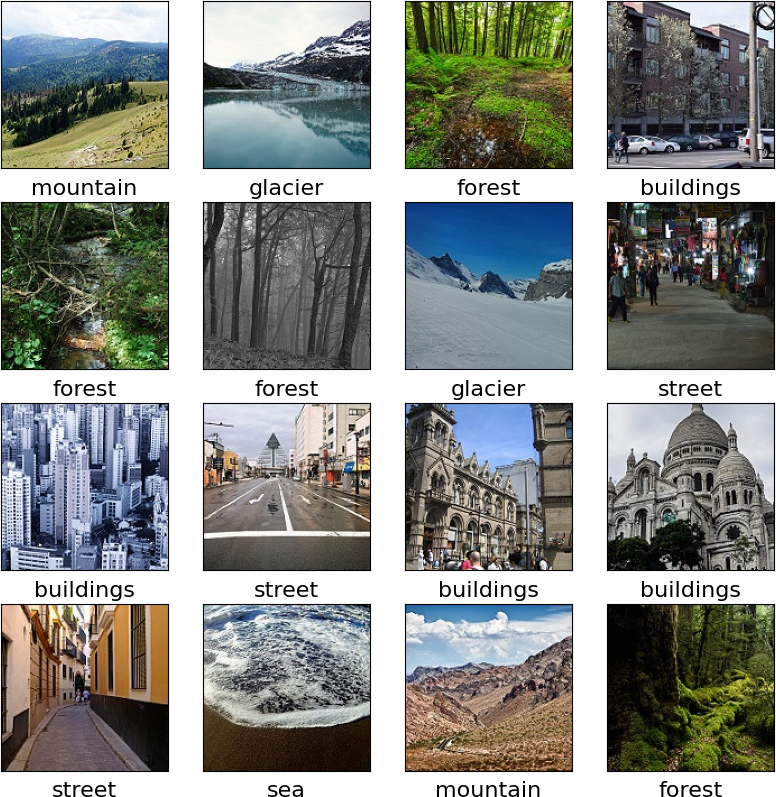
\includegraphics[width=2.5in]{../images/samples.png}
\captionsetup{justification=centering}                                                                                         
\caption{$16$ random entries of the train dataset}
\label{fig:samples}                                                                                                                               
\end{figure}

The distribution of the images across the classes follows a uniform distribution $U(\mu, \sigma)$: in the train set each class has an average $\mu = 2\,339$ images with $\sigma = 105.45$ and in the test set $\mu=500$ and $\sigma=36.92$. We didn't find any bias inside the dataset since all the classes are equally populated and so we didn't applied any kind of data augmentation on particular classes for rebalacing.


\begin{figure}[ht!]
\centering                                                                        
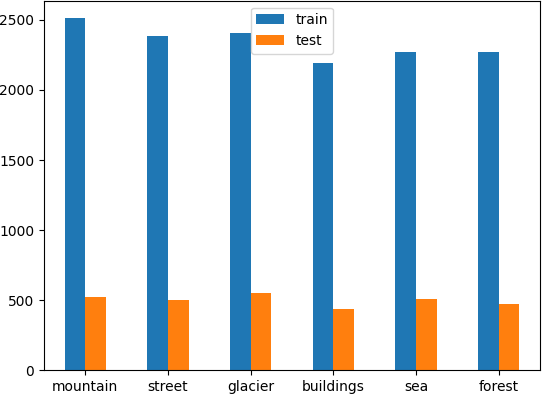
\includegraphics[width=3in]{../images/data.png}
\captionsetup{justification=centering}                                                                                         
\caption{16 entries of the train dataset}
\label{fig:data}                                                                                                                               
\end{figure}

The $6$ classes are encoded with numbers $0$ to $5$ and Table \ref{tab:encode} shows the mapping between the numerical and nominative form.



\begin{table}[ht!]
\centering
\begin{tabular}{|l|l|}
\hline
\rowcolor[HTML]{9698ED} 
{\color[HTML]{FFFFFF} \textbf{Number}} & {\color[HTML]{FFFFFF} \textbf{Class}} \\ \hline
0                                      & Building                              \\ \hline
1                                      & Forest                                \\ \hline
2                                      & Glacier                               \\ \hline
3                                      & Mountain                              \\ \hline
4                                      & Sea                                   \\ \hline
5                                      & Street                                \\ \hline
\end{tabular}
\caption{Mapping between numbers and names}
\label{tab:encode}
\end{table}







\bibliographystyle{ieeetr}
\bibliography{Bibliography}

\begin{thebibliography}{9}

\bibitem{site1} 
Practice Problem: Intel Scene Classification Challenge \\
\texttt{https://datahack.analyticsvidhya.com/contest/practice-problem-intel-scene-classification-challe}

\bibitem{site2} 
OpenVINO™ documentation \\
\texttt{https://docs.openvino.ai/latest/index.html}



\end{thebibliography}

\end{document}









